% -*- TeX -*-
%
% ----------------------------------------------------------------------
%
%                           Brad T. Aagaard
%                        U.S. Geological Survey
%
% {LicenseText}
%
% ----------------------------------------------------------------------
%
\documentclass[pdftex,cig,slideColor]{pp4slides}
\usepackage{amsmath}
\usepackage{array}
\usepackage{xspace}
\usepackage{multirow}
\usepackage{ulem}

\newcommand{\newfeature}[1]{{\color{blue}#1}}

\renewcommand{\movielink}[2]{\href{run:#1.avi}{#2}}

\title{Community Benchmarks for Code Verification}
\author{Brad Aagaard}
\institution{\includegraphics[height=2cm]{../../logos/cig}}
\date{June 17, 2010}

% --------------------------------------------------------- DOCUMENT
\begin{document}

% ------------------------------------------------------------ SLIDE
\maketitle

% ------------------------------------------------------------ SLIDE
\foilhead{Community Benchmarking Efforts}
  \summary{}

 \begin{itemize}
 \item SCEC Crustal Deformation Modeling (quasi-static)
   \begin{itemize}
   \item Focus on geometry, viscoelastic rheology, quantifying error
   \item Very few codes (PyLith and GeoFEST)
   \item Large benchmark suite $\Rightarrow$ small benchmark suite
   \end{itemize}
 \item SCEC Earthquake Source Physics (dynamic)
    \begin{itemize}
    \item Focus on geometry, elastic/elastoplastic, qualitative
      comparison
    \item More than a dozen codes
    \item 1--2 benchmark problems per year
    \end{itemize}
  \end{itemize}

\bgadd{\vspace*{7.9in}%
  \begin{center}%
    \includegraphics[height=14mm]{../../logos/cig}
  \end{center}}


% ------------------------------------------------------------ SLIDE
\foilhead{Summary of Community Benchmarks}
  \summary{}

{\small
  \begin{center}
    \begin{tabular}{lccc}
      Category & Rheology & Fault geometry & Fault model \\ \hline
      SCEC Crustal & Maxwell viscoelastic & vertical, strike slip & kinematic \\
      Deformation & & dipping, reverse slip & \\
      Modeling & w/gravity & dipping, reverse slip & \\
      & & vertical, strike slip & eq cycle \\ \hline
      SCEC Eq & elastic & vertical, strike slip & slip weakening \\
      Source & w/bi-material & vertical, strike slip & slip weakening \\
      Physics &            & vertical, strike slip & overburden press. \\
              &            & dipping, normal slip & subshear \\
              &            & dipping, normal slip & supershear \\
              & Drucker-Prager & dipping, normal slip & overburden press. \\
              & elastic & vertical, strike slip & rate and state \\ \hline
   \end{tabular}
  \end{center}
}
  
% ------------------------------------------------------------ SLIDE
\foilhead{Quasi-static: Strike-Slip Benchmark}
  \summary{}


  \vfill
  \begin{center}
    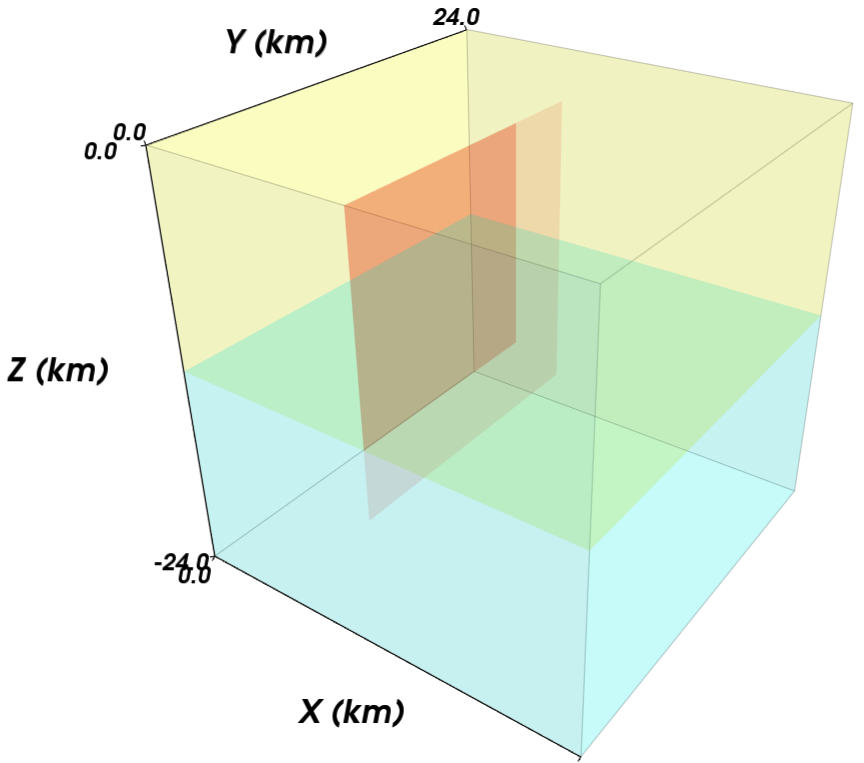
\includegraphics[scale=0.55]{figs/strikeslipnog_geometry}
  \end{center}
  \vfill


% ------------------------------------------------------------ SLIDE
\foilhead{Quasi-static: Strike-Slip Benchmark}
  \summary{}


  \vfill
 \begin{center}
    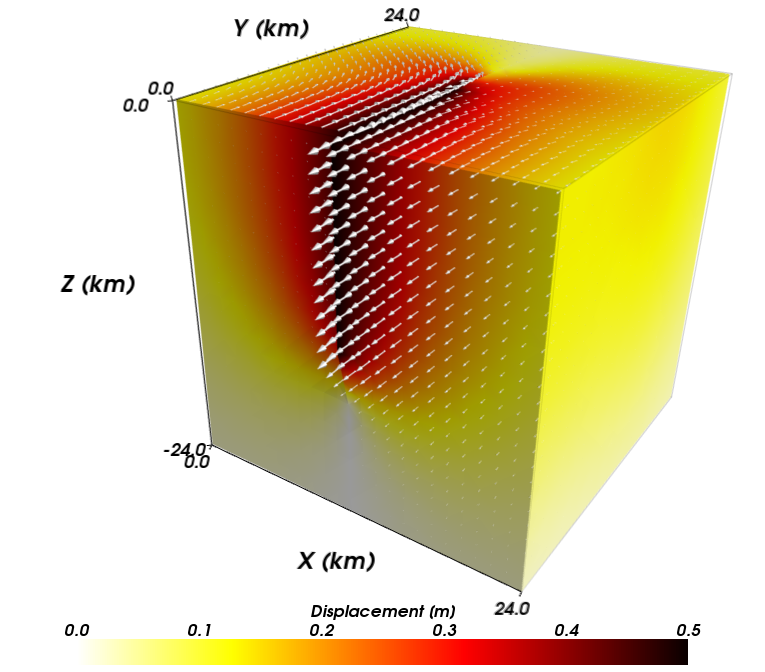
\includegraphics[scale=0.65]{figs/strikeslipnog_soln}
  \end{center}
  \vfill


% ------------------------------------------------------------ SLIDE
\foilhead{Quasi-static: Strike-Slip Benchmark}
  \summary{Error metric}

  \begin{itemize}
  \item Local error
    \begin{equation}
      E_\mathit{local} = \frac{1}{V_\mathit{cell}}
        \sqrt{\int_\mathit{cell} \left( u_i^A - u_i^B \right)^2 \, dV}
    \end{equation}
  \item Global error
    \begin{equation}
      E_\mathit{domain} = \frac{1}{V_\mathit{domain}}
        \sqrt{\int_\mathit{domain} \left( u_i^A - u_i^B \right)^2 \, dV}
    \end{equation}
  \end{itemize}
  
% ------------------------------------------------------------ SLIDE
\foilhead{Quasi-static: Strike-Slip Benchmark}
  \summary{Error for Hex8, 1000m resolution}


  \vfill
 \begin{center}
    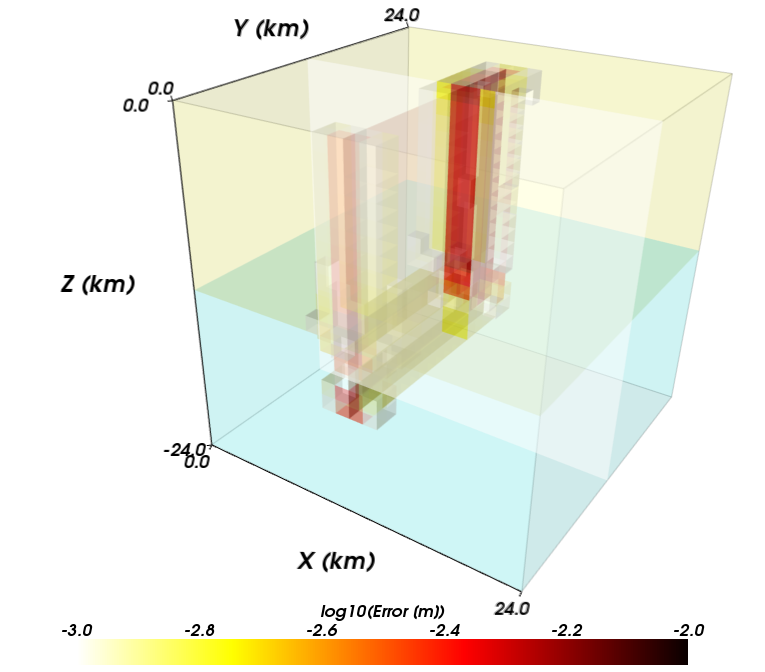
\includegraphics[scale=0.65]{figs/strikeslipnog_err_hex8_1000m}
  \end{center}
  \vfill


% ------------------------------------------------------------ SLIDE
\foilhead{Quasi-static: Strike-Slip Benchmark}
  \summary{Error for Hex8, 500m resolution}


  \vfill
 \begin{center}
    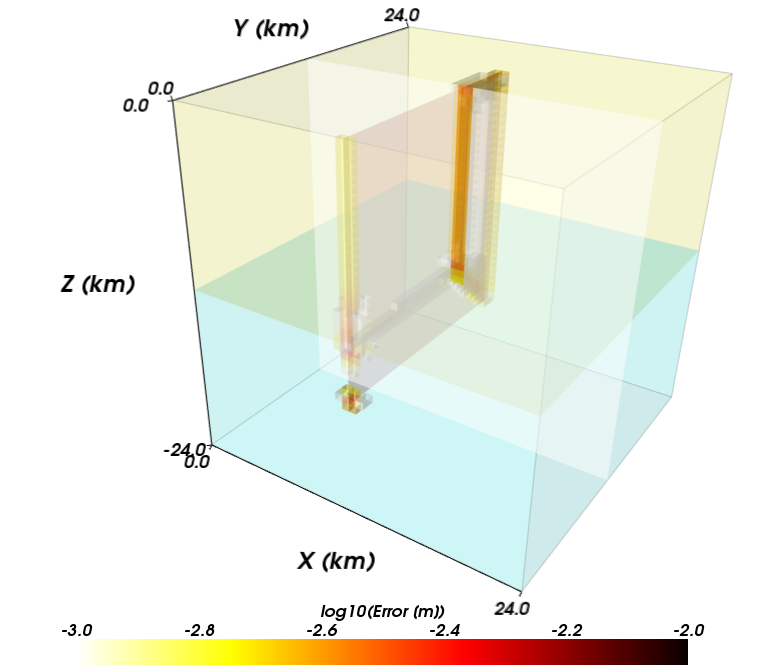
\includegraphics[scale=0.65]{figs/strikeslipnog_err_hex8_0500m}
  \end{center}
  \vfill


% ------------------------------------------------------------ SLIDE
\foilhead{Quasi-static: Strike-Slip Benchmark}
  \summary{Error for Hex8, 250m resolution}


  \vfill
 \begin{center}
    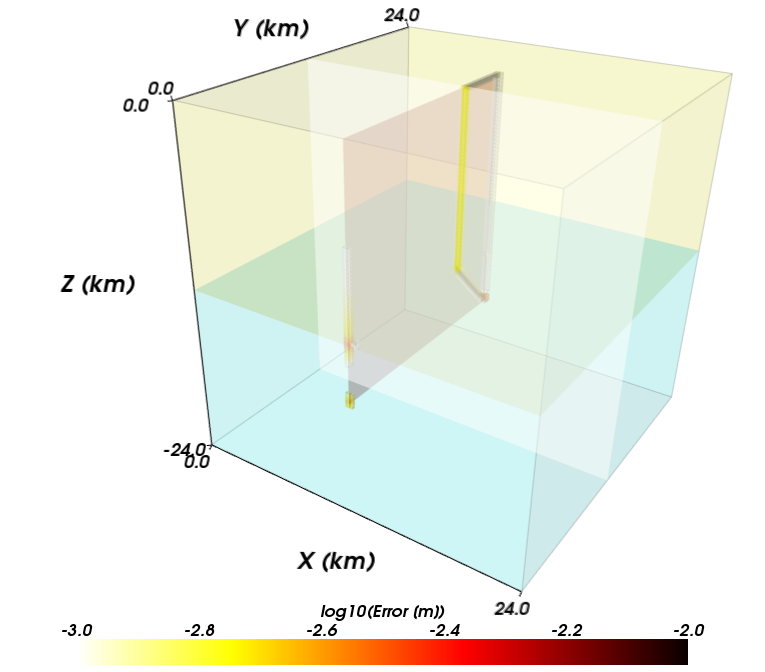
\includegraphics[scale=0.65]{figs/strikeslipnog_err_hex8_0250m}
  \end{center}
  \vfill


% ------------------------------------------------------------ SLIDE
\foilhead{Quasi-static: Strike-Slip Benchmark}
  \summary{Error for Tet4, 1000m resolution}


  \vfill
 \begin{center}
    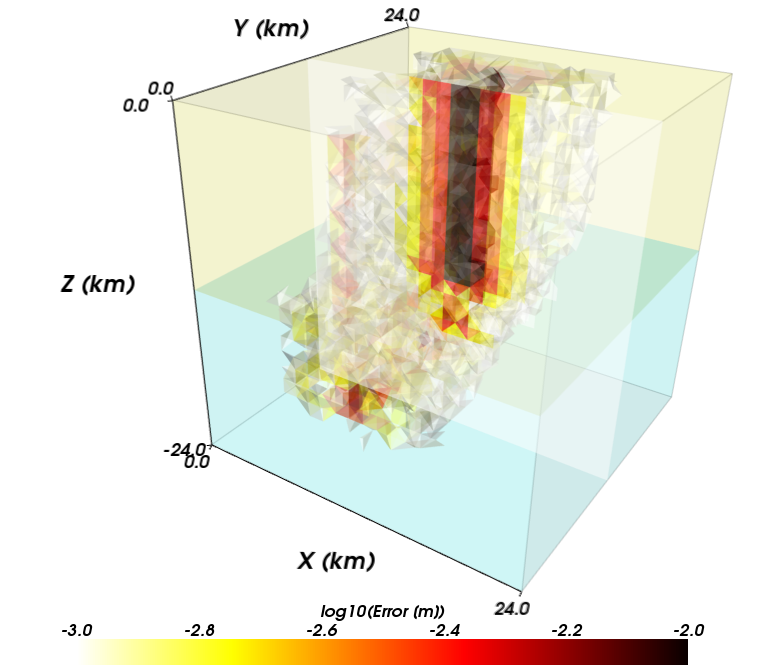
\includegraphics[scale=0.65]{figs/strikeslipnog_err_tet4_1000m}
  \end{center}
  \vfill


% ------------------------------------------------------------ SLIDE
\foilhead{Quasi-static: Strike-Slip Benchmark}
  \summary{Error for Tet4, 500m resolution}


  \vfill
 \begin{center}
    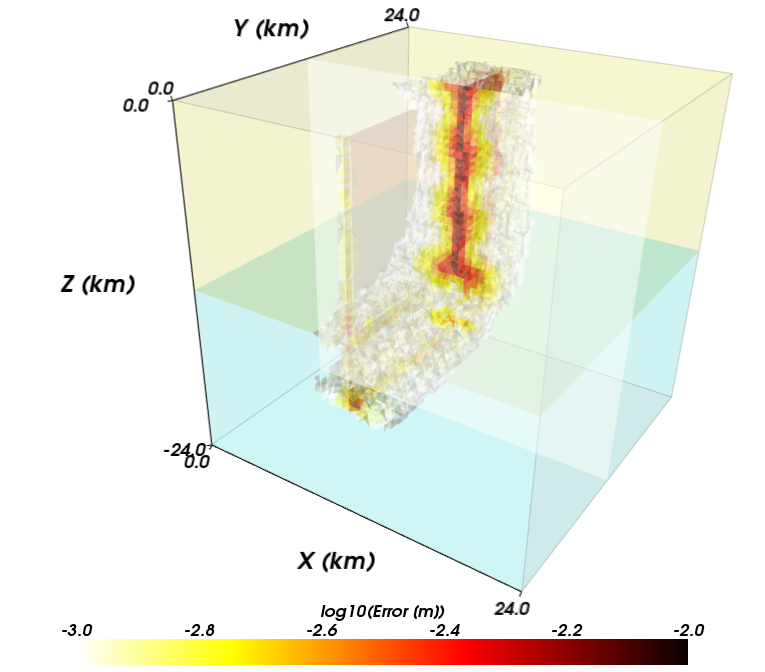
\includegraphics[scale=0.65]{figs/strikeslipnog_err_tet4_0500m}
  \end{center}
  \vfill


% ------------------------------------------------------------ SLIDE
\foilhead{Quasi-static: Strike-Slip Benchmark}
  \summary{Error for Tet4, 250m resolution}


  \vfill
 \begin{center}
    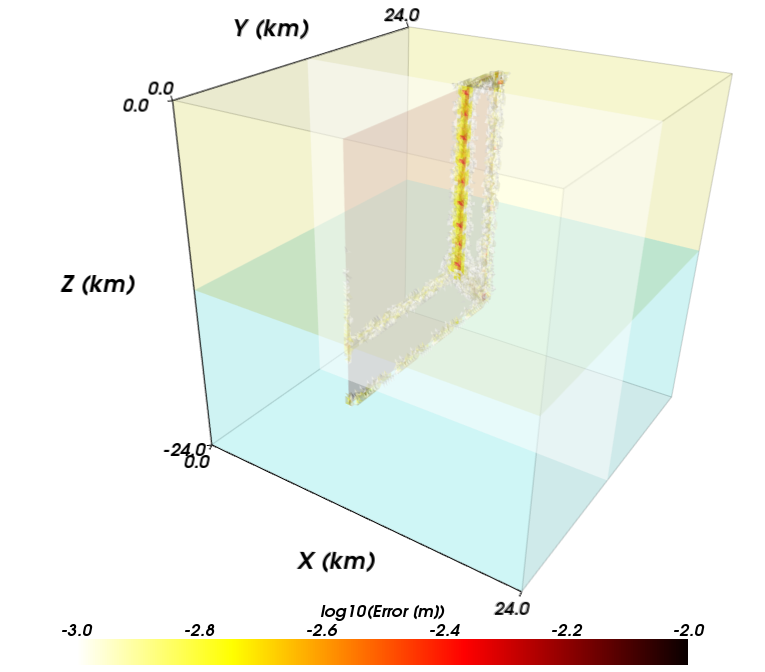
\includegraphics[scale=0.65]{figs/strikeslipnog_err_tet4_0250m}
  \end{center}
  \vfill


% ------------------------------------------------------------ SLIDE
\foilhead{Quasi-static: Strike-Slip Benchmark}
  \summary{Hex8 outperforms Tet4}


  \vfill
 \begin{center}
    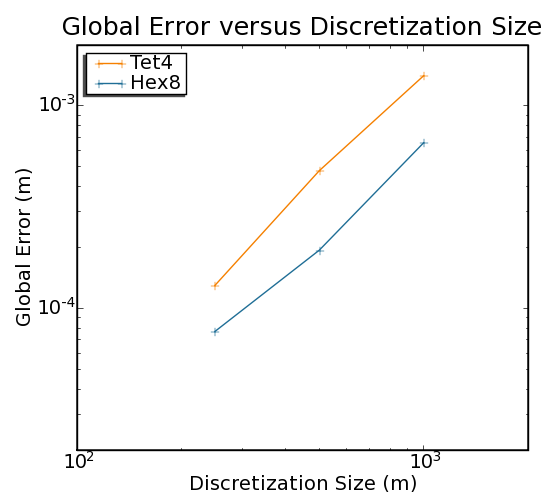
\includegraphics[scale=0.8]{figs/strikeslipnog_convergence}
  \end{center}
  \vfill


% ------------------------------------------------------------ SLIDE
\foilhead{Quasi-static: Savage-Prescott Benchmark}
  \summary{}


  \vfill
  \begin{center}
    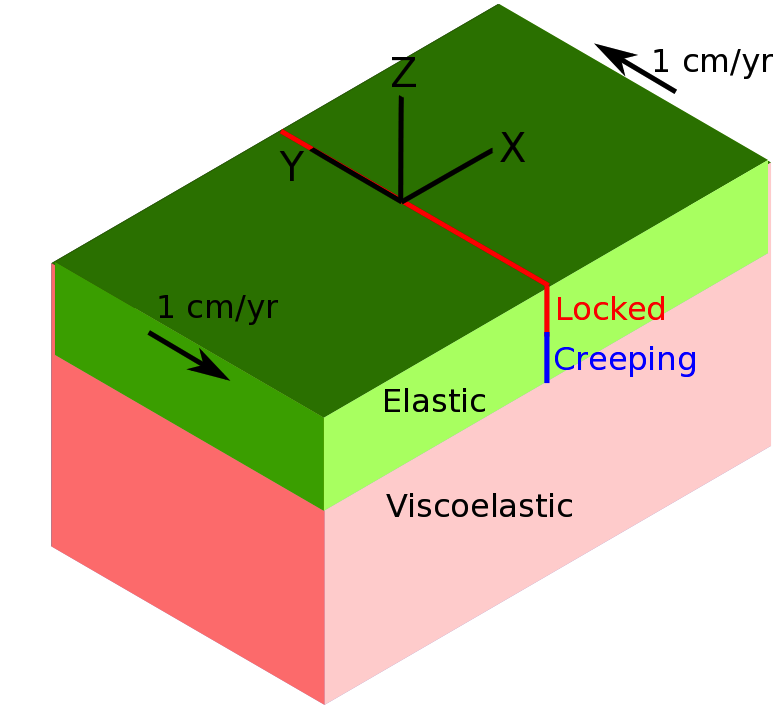
\includegraphics[scale=0.6]{figs/savageprescott_geometry}
  \end{center}
  \vfill


% ------------------------------------------------------------ SLIDE
\foilhead{Quasi-static: Savage-Prescott Benchmark}
  \summary{}


  \vfill
  \begin{center}
    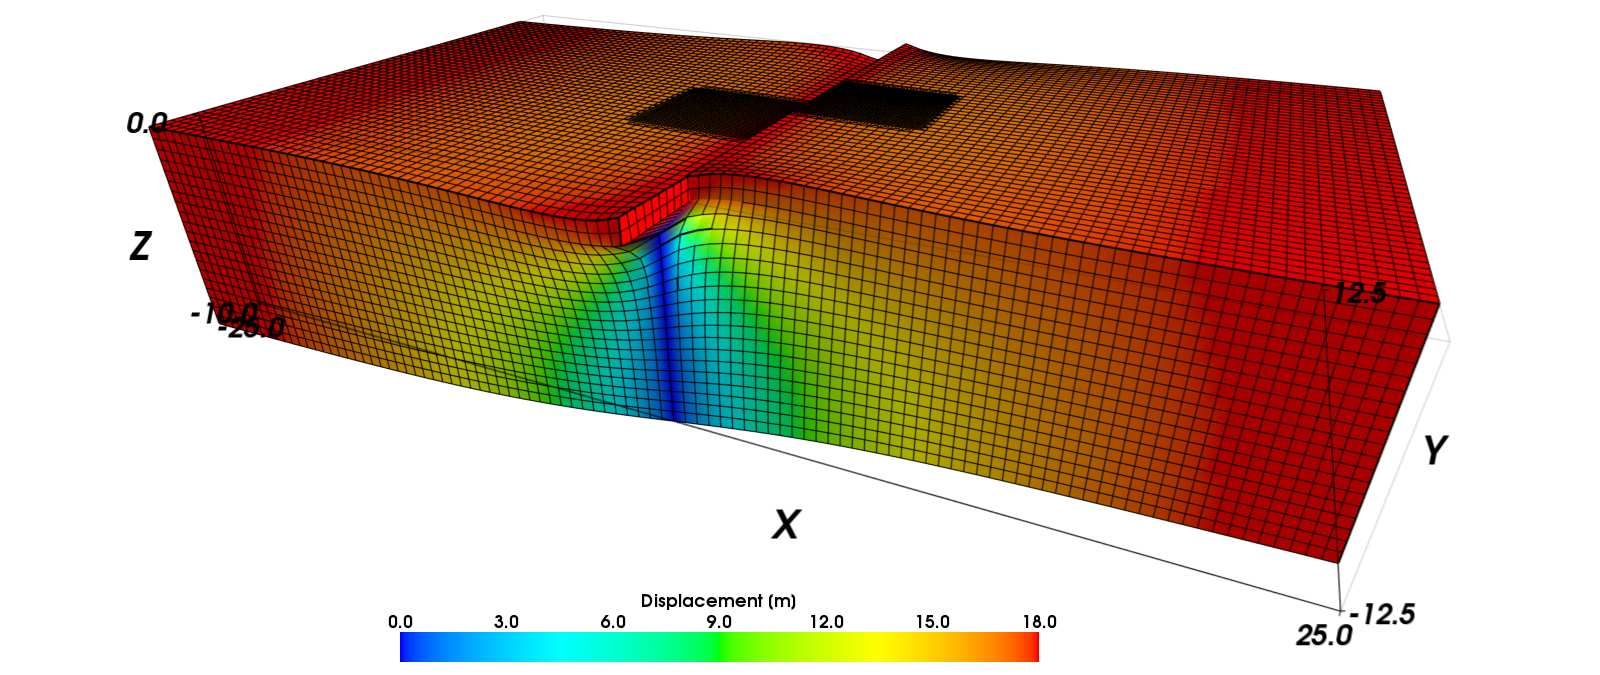
\includegraphics[scale=0.8]{figs/savageprescott_soln}
  \end{center}
  \vfill


% ------------------------------------------------------------ SLIDE
\foilhead{Quasi-static: Savage-Prescott Benchmark}
  \summary{Analytic versus PyLith: Earthquake cycle 3}

  \vfill
  Model has not yet spun-up to steady-state solution.

  \vfill
  \begin{center}
    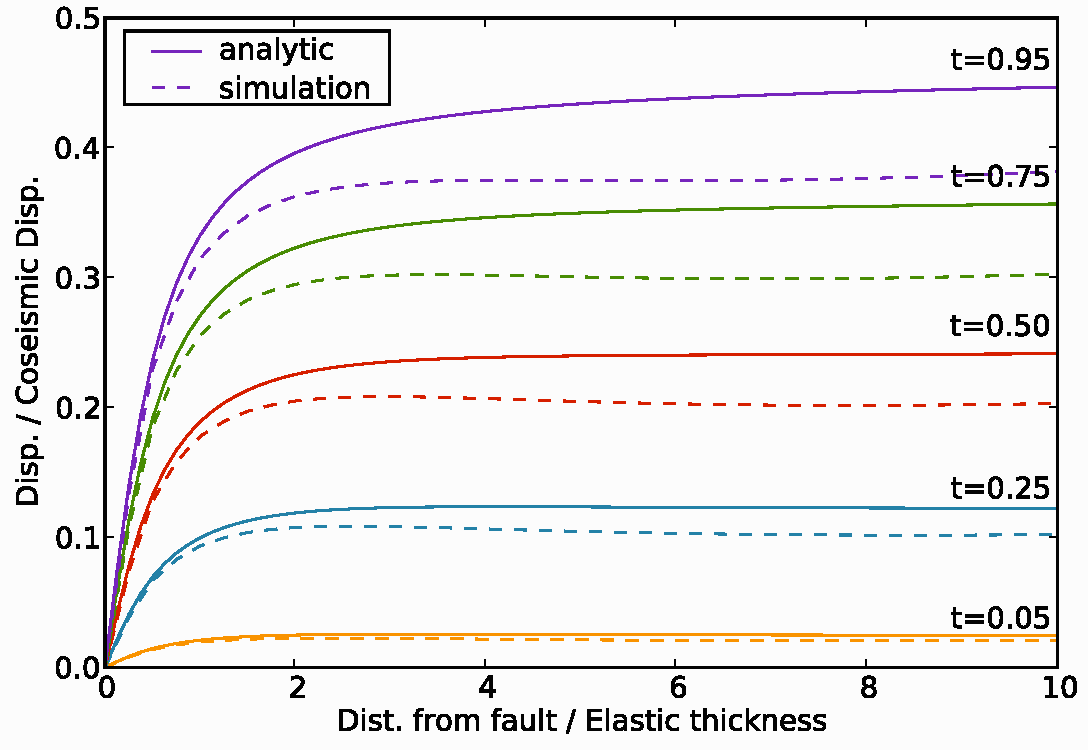
\includegraphics[scale=0.8]{figs/savageprescott_profile2}
  \end{center}
  \vfill


% ------------------------------------------------------------ SLIDE
\foilhead{Quasi-static: Savage-Prescott Benchmark}
  \summary{Analytic versus PyLith: Earthquake cycle 10}

  \vfill
  Model is very close to steady-state solution.

  \vfill
  \begin{center}
    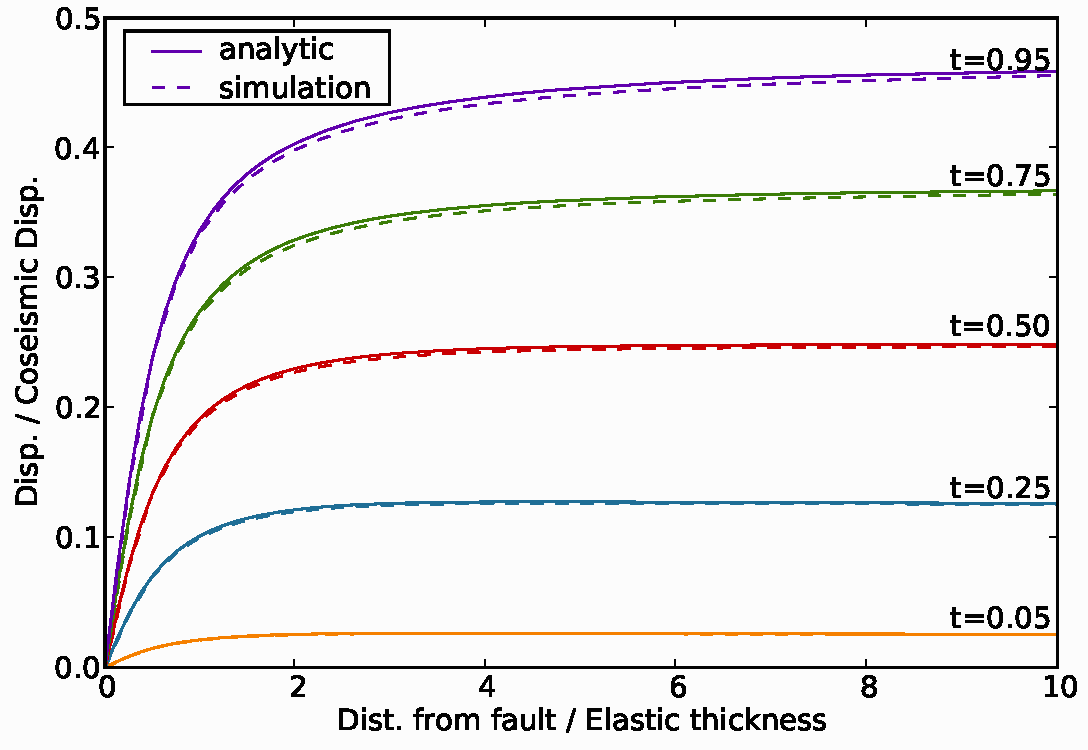
\includegraphics[scale=0.8]{figs/savageprescott_profile9}
  \end{center}
  \vfill


% ------------------------------------------------------------ SLIDE
\foilhead{Quasi-static Benchmarks: What is missing?}
  \summary{Need benchmarks for new features}

  \begin{itemize}
  \item PyLith features not tested by benchmarks
    \begin{itemize}
    \item Power-law quasi-static
    \item Small strain (have full-scale tests for rigid body motion)
    \item Drucker-Prager quasi-static
    \item Generalized Maxwell
    \item Quasi-static w/friction
    \end{itemize}
  \item New benchmarks
    \begin{itemize}
    \item Code comparison based on current benchmarks for new features
      \begin{itemize}
      \item Strike-slip benchmark w/power-law rheology?
      \item Savage-Prescott benchmark w/power-law rheology?
      \end{itemize}
    \item Verification w/analytical and semi-analytical solutions
    \end{itemize}
 \end{itemize}
  

% ======================================================================
\end{document}


% End of file
